% 记录阅读文献时遇到的一些数学概念等
\subsection{采样}
采样是生成一堆数据的过程,如果最终生成的数据服从某个分布,则可以称这堆数据采样自这个分布。
\subsubsection{alias sampling }
一种高效的针对\textbf{离散概率分布}采样方法,但是要先经过预处理,预处理的时间为$O(n)$,但是与处理完成后采样的时间时$O(1)$。预处理的大致思路如下:\\
对于一个给定的离散概率分布:$p(X = x_i) , X = x_1, x_2, ..., x_n$。按照序号构造n个盒子,每个盒子按照顺序一一与$x_1, ..., x_n$对应,每个盒子的高度为$n \cdot p(X = x_i)$。接下来通过取长补短,把高度高于1的盒子切一部分分到其他高度低于1的盒子上,而且每个序号对应处不能有超过两个盒子。所以需要两个数组(Alias,Accept)来记录预处理的结果,一个用来记录每个序号除了原来的盒子还放了哪个盒子,一个用来记录每个序号的外来盒子有多高。\\
进行采样时,先决定使用哪个序号对应的盒子,再决定使用该序号内的原来的盒子还是外来的盒子。一个简单的例子Fig.\ref{fig:alias-sample}
\begin{figure}[h]
	\centering
	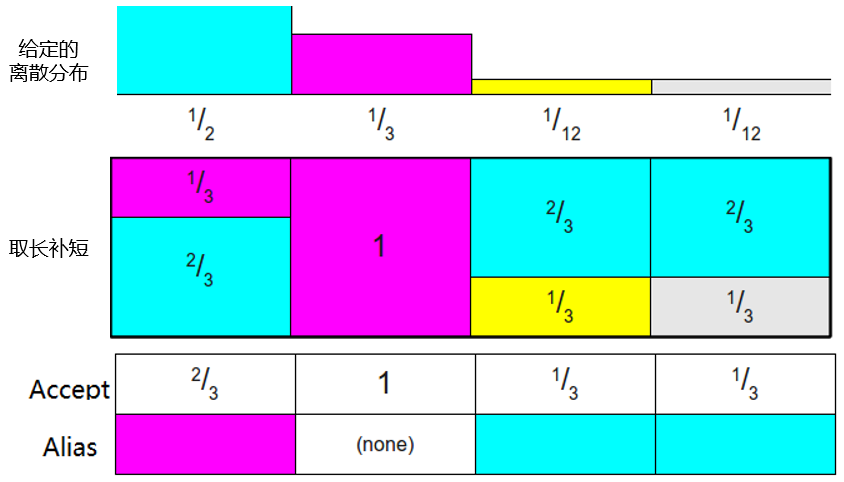
\includegraphics[width=.8\textwidth]{pics/alias-sample.png}
	\label{fig:alias-sample}
	\caption{Alias Sample例子}
\end{figure}


参考资料:
\begin{enumerate}
    \item \href{https://www.keithschwarz.com/darts-dice-coins/}{Darts, Dice, and Coins: Sampling from a Discrete Distribution}
    \item \href{https://www.cnblogs.com/dogecheng/p/13198198.html}{【图嵌入】DeepWalk 和 Node2Vec}
\end{enumerate}

\subsubsection{Importance Sampling}
重要性采样,一种近似的抽样方法, 通过一些数学上的变化, 使得可以对一些不好抽样的分布进行抽样和估计。这个会在强化学习中的off-policy的方法中用到, 从一个策略进行抽样, 更新另外一个策略。求函数$f(x)$的积分可以写成求期望的形式:
$$
E_{x \sim p(x)}[f(x)] = \int p(x) f(x) d x \approx \frac{1}{n} \sum_{i} f(x_{i})
$$
然而通常数据分布会比较复杂且积分也是一个复杂的过程,因此会用采样来代替之。上式中的第三项就是用采样来代替积分,其中$\frac{1}{n}$表示$p(x) = \frac{1}{n}$,即数据的分布。但是有时候$p(x)$是个很复杂的分布,从其重采样是很困难的,这个时候该怎么办呢?

找一个已易于采样的分布$q(x)$,如正态分布,从$q(x)$中采样得到的很多样本作为从$p(x)$中采样的样本集,那么问题就来了,这俩又不是同一个分布,$q(x)$中采样的样本集分布符合$p(x)$吗?先看一个公式:
$$
E_{x \sim p(x)}[f(x)] = \int q(x) \frac{p(x)}{q(x)} f(x) d x \approx \frac{1}{n} \sum_{i}  \frac{p(x)}{q(x)} f(x_{i})
$$
这个就是当我们从$q(x)$中采样代替$p(x)$后求$f(x)$积分/期望的公式。可以看出对于从$q(x)$中采样的样本赋予了不同的权重,因为样本集来自$p(x)$的概率是不一样的,其中重要性就是$\frac{p(x)}{q(x)}$。如Fig.\ref{fig:importance-sample}所示。注意:图中$p(z)$与$f(z)$的含义,$p(z)$是一种分布,是相对于$z$轴的采样点而言的,比如在红色的两个驼峰处,$z$的取点比较多,在其他地方$z$的取点就比较少,这叫样本分布服从$p(z)$。对于$f(z)$是一种映射关系,将$z$值映射到其他维度。

\begin{figure}[h]
	\centering
	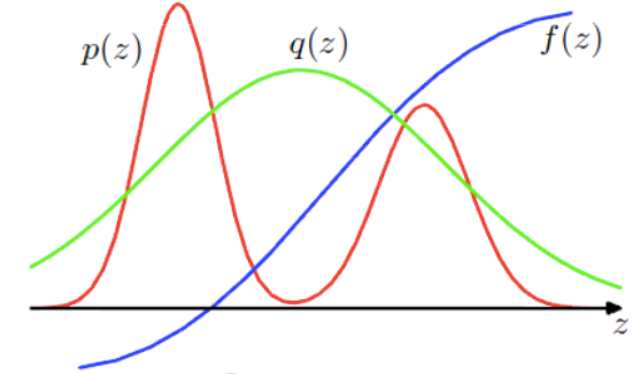
\includegraphics[width=.5\textwidth]{pics/importance-sample.png}
	\label{fig:importance-sample}
	\caption{重要性采样}
\end{figure}

参考:\href{https://www.jianshu.com/p/3d30070932a8}{随机模拟-Monte Carlo积分及采样(详述直接采样、接受-拒绝采样、重要性采样)}。


\subsubsection{接受-拒绝采样}
同样的问题:对于一个难以采样的分布$p(x)$,该怎么采样呢?选择一个易于采样的分布$q(x)$,从中采样,以一定的概率接受或拒绝采样到的样本,使得经过筛选后的样本集是服从$p(x)$的。
\begin{figure}[h]
	\centering
	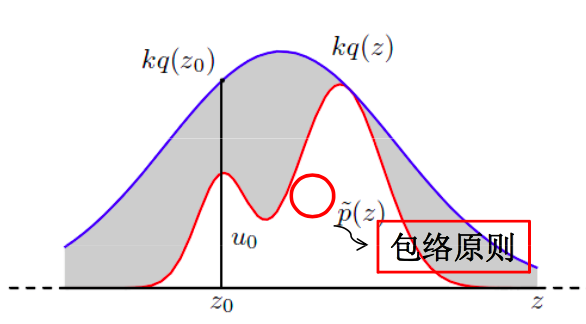
\includegraphics[width=.6\textwidth]{pics/accept-reject-sample.png}
	\label{fig:accept-reject-sample}
	\caption{接受-拒绝采样}
\end{figure}
具体该怎么操作呢?如Fig.\ref{fig:accept-reject-sample}所示,选择$q(x)$,乘以$k$得到$kq(x)$使之刚好能够保住$p(x)$。对于$q(x)$中采样到的样本$z_0$,从$[0, 1]$的均匀分布中取一个数$u_0$,如果$u_0 \le \frac{p(z_0)}{q(z_0)}$则接受$z_0$。

\subsection{eigen-value \& eigen—vector }
特征值,特征向量。
这两者到底有什么意义呢?


\subsection{Density estimation }

\subsection{MMD}
Maximum mean discrepancy。 用来衡量两个分布的差异。具体的衡量过程是:
假设有两个分布p, q,那么利用这两个分布分别生成两个样本集ps, qs,再假设有一个函数f,对于$pm = \sum_{i \in ps}f(i), qm = \sum_{j \in qs}f(j) $,
则分布p, q 在f上的MMD为 $pm$与$qm$的差或某种基于$pm, qm$ 的计算值。

\subsection{P, NP, NP-hard}
P问题:确定性计算机能够在指数级时间解决的问题;

NP问题:非确定性计算机能够在指数级时间解决的问题;

NPC问题:存在这样一个NP问题,所有NP问题都能约化成它,即只要解决了这个问题则所有NP问题都能解决。NPC需要满足两个条件:
\begin{itemize}
	\item 它是一个NP问题
	\item 所有的NP问题都能规约到它
\end{itemize}

NP-hard问题:满足NPC问题的第二个条件,但不一定满足第一条。NP-hard问题同样难以找到多项式时间的解法,但不一定是NP问题。这几者之间的包含关系如\ref{fig:P-NP-NPC-NP-hard}所示。

\begin{figure}[h]
	\centering
	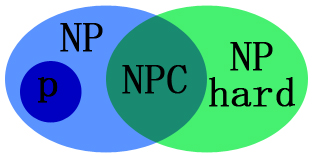
\includegraphics[width=.4\textwidth]{pics/P-NP-NPC-NP-hard.jpeg}
	\caption{P\_NP\_NPC\_NP-hard}
	\label{fig:P-NP-NPC-NP-hard}
\end{figure}



\subsection{傅里叶变换和小波分析}
傅里叶变换:知道一段时间内,信号的各个频率分量分别有多少。
小波变换:知道一段时间内,信号的各个频率分量分别有多少,以及它们都是什么时候出现的。

参考资料:\href{https://cseweb.ucsd.edu/~baden/Doc/wavelets/polikar_wavelets.pdf}{《The Wavelet Tutorial》}、\href{https://www.zhihu.com/question/22864189/answer/40772083}{如何通俗地讲解傅立叶分析和小波分析间的关系? - 咚懂咚懂咚的回答}。

\subsection{$l_1, l_2$范数对最优化问题的影响}
考虑以下优化问题:
\begin{equation}
	\begin{aligned}
		\min _{x \in \mathbb{R}^{n}} &\|x\|_{p}, \\
		\text { s.t. } & A x=b \label{eq-opt}
	\end{aligned}
\end{equation}
公式.\ref{eq-opt}中$p$表示0,1,2,$\|x\|_{p}$表示$x$的$l_p$范数。
在深度学习中,通常希望得到稀疏的解(稀疏的解,对数据的扰动也更鲁棒),即在满足约束的情况下,$x$中的非零值的数量尽可能多。咋一看,可能$l_0$范数是最符合情况的,但是$\|x\|_0$是不连续的,当$p=0$时,公式.\ref{eq-opt}就成了NP问题。当$A, b$满足一定条件时,$p=1$的时公式.\ref{eq-opt}的解也是$p=0$时的解。$l_1$范数优化问题更易求解。那么有没有更容易求解的范数呢,$l_2$可以吗?

对公式.\ref{eq-opt}进行转化:由于范数本身也是函数,该优化问题就可以视为在$A x = b$的约束下,$\|x\|_p$的最小值,从函数图像角度来看这个优化问题,就是\textbf{目标函数与约束函数的交集 --- 相交时的最小值}。

当$x \in \mathbb{R}^2$时,如Fig.\ref{fig:norm optimize}所示。
\begin{figure}[h]
	\centering
	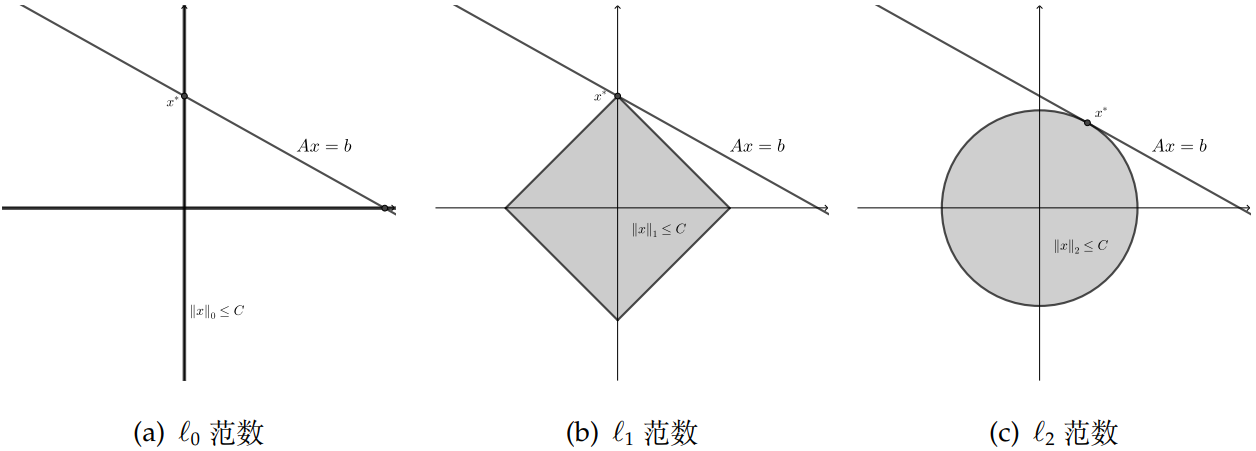
\includegraphics[width=.85\textwidth]{pics/norm optimize.png}
	\caption{$l_0, l_1, l_2$范数优化问题求解示意图}
	\label{fig:norm optimize}
\end{figure}
对$l_0$范数,$\{x | \|x\|_0 \leq 2\}$是全平面,它自然与$A x = b$相交;$\{x | \|x\|_0 \leq 1\}$退化成两条直线即坐标轴,此时问题的解就是$A x = b$与坐标轴的交点。
\begin{itemize}
	\item 对$l_1$范数,根据$C$不同,$\{x | \|x\|_1 \leq C\}$为一系列正方形,这些正方形的顶点落在坐标轴上,$A x = b$与这些正方形的交点一般是在正方形的顶点即相交于坐标轴,因此$l_1$范数的解有稀疏性
	\item 对$l_2$范数,根据$C$不同,$\{x | \|x\|_1 \leq C\}$为一系列圆,且圆有光滑的边界,圆和$A x = b$的交点可以是圆上任何一点,所以$l_2$范数优化问题一般不能保证解的稀疏性
	\item 对$l_2$范数,根据$C$不同,$\{x | \|x\|_1 \leq C\}$为一系列圆,且圆有光滑的边界,圆和$A x = b$的交点可以是圆上任何一点,所以$l_2$范数优化问题一般不能保证解的稀疏性
\end{itemize}

注意:\tbc{red}{这里目标函数与约束函数相交一般是指相切,$\{x | \|x\|_p \leq C\}$可以看成一个广义的球体,如果该球体与$A x = b$相交而不是相切,那么一定存在一个更小的$C'$使$\|x\|_p$更小且与$A x = b$相切,则$C'$成了比$C$更优的解,故一般考虑相切。}

参考资料:
\begin{itemize}
	\item《最优化:建模、算法与理论》,刘浩洋、户将、李勇锋、文再文编著,第一章,1.2
	\item \href{https://blog.csdn.net/red_stone1/article/details/80755144}{机器学习中 L1 和 L2 正则化的直观解释}
\end{itemize}


\subsection{Reparametrization}重参数化技术。参考:\href{https://spaces.ac.cn/archives/6705}{漫谈重参数:从正态分布到Gumbel Softmax}

\subsection{常用统计量}
\subsubsection{方差(Variance)} 一组数据的方差,描述的是数据与它们的均值的离散程度,衡量了这组数据的集中程度。方差可以分为样本方差和总体方差:
\begin{itemize}
	\item 样本方差:$S^2 = \frac{\sum_{i=1}^N(x_i - \bar{x})^2}{N-1}$,其中$\bar{x}$是\textbf{样本均值}
	\item 总体方差:$\sigma^2 = \frac{\sum_{i=1}^N(x_i - \mu)^2}{N}$,其中$\mu$是\textbf{总体均值}
\end{itemize}
\textbf{为什么不用要平方?}如果使用平均差($\frac{\sum_{i=1}^N |x_i - \bar{x}|}{N}$)来衡量一组数据的离散程度,可能不能很好的体现数据的分散程度(参考:\href{https://www.shuxuele.com/data/standard-deviation.html#WhySquare}{为什么要求差的平方?}),加上平方后可以放大偏离均值太远的数据的影响。也许这有点像注意力机制,在平均差中,$|x_i - \bar{x}|$的注意力值是$\frac{1}{N}$,在方差中,$|x_i - \bar{x}|$的注意力值是$\frac{|x_i - \bar{x}|}{N}$,这可以体现离均值越远的点对离散程度的贡献越大。

\subsubsection{标准差(Standard Deviation)} 标准差的平方就是方差,同理,标准差也可以分为样本std.和总总体std.:
\begin{itemize}
	\item 样本标准差:$S = \sqrt{S^2}$
	\item 总体标准差:$\sigma = \sqrt{\sigma^2}$
\end{itemize}

\subsubsection{T-statistic }


\subsubsection{p-value }

\subsubsection{t test、$\chi^2$检验}
$\chi^2$检验通常用于检验两个事件的独立性,例如可以用于分析自变量与因变量之间的独立性。如果$\chi^2$的值越大,则说明二者之间的关联性越大。

\subsection{数据的度量}
\subsubsection{定类变量}
即类别变量,其值域是某个离散的类别。能够对对象进行分类,能够判断对象之间是否同类或异类,如性别。\tbc{red}{不同类别之间没有大小关系}。

\textbf{【可以分类( $=$ 和 $\neq$),但不能排序】}

\subsubsection{定序变量}
定序变量的值不仅能够代表事物的分类,还能代表事物按某种特性的排序,但定序变量的值之间没有确切的间隔距离,\tbc{red}{只能排列出它们的顺序,而不能反映出不同值之间的距离},即不能反映一个值比另一个值大多少或小多少。如文化水平,其取值可以是文盲、小学、中学、大学等,值之间有顺序关系(如大学 $\textgreater$ 小学),但不能反映不同文化程度之间的距离。

\textbf{【可以分类( $=$ 和 $\neq$),可以排序($\textgreater$ 和 $\textless$),但不能($+$ 和 $-$ )】}

\subsubsection{定距变量}
定距变量的值之间\tbc{red}{可以比较大小,两个值的差有实际意义}。能确切测量值之间的高低、大小次序之间的距离,因而具有加与减的数学特质。但是,\tbc{red}{定距变量没有一个绝对的零点},不能乘除或倍数的形式来说明它们之间的关系。例如华氏温度:10、20、30,30比20高10,但华氏度30不是10的三倍热(\tbc{red}{0不是没有温度})。

\textbf{【可以分类( $=$和 $\neq$ ),可以排序($\textgreater$ 和 $\textless$),可以($+$ 和 $-$ ),但不能($\times$和 $\div$ )】}

\subsubsection{定比变量}
定比变量除了具有定距变量的特性外,还具有一个真正的零点,因而它具有乘与除(×、÷)的数学特质。如A的体重是60kg,而B的体重是30kg,可以算出前者是后者的两倍重,因为其零点是绝对的。

\textbf{【可以分类( $=$和 $\neq$ ),可以排序($\textgreater$ 和 $\textless$),可以($+$ 和 $-$ ),可以($\times$和 $\div$ )】}

以上四种变量类型的性质是逐渐继承的。

参考:\href{https://blog.csdn.net/YYIverson/article/details/100068865}{【统计学】区分定类、定序、定距、定比变量!!}。

\subsection{拉格朗日对偶性}
约束最优化中常用的一种方法。利用拉格朗日对偶性(Lagrange duality)将原始问题转换为对偶问题,通过求解对偶问题得到原始问题的解。

\subsubsection{原始问题}假设$f(x), g_i(x), h_j(x)$是定义在$\mathbb{R}^n$的连续可微函数。原始最优化问题为:
\begin{align}
	\mathop{min}_{x \in \mathbb{R}^n}&\quad f(x) \nonumber \\
	s.t.&\quad g_i(x) \leqslant 0, i = 1, 2, ..., k \nonumber \\
		&\quad h_j(x) = 0, j = 1, 2, ..., l \nonumber
\end{align}

引进广义朗格朗日函数:
$$
L(x, \alpha, \beta) = f(x) + \sum_{i=1}^k a_i g_i(x) + \sum_{i=j}^l \beta_j h_j(x)
$$
其中,$x \in \mathbb{R}^n$,$\alpha, \beta$是拉格朗日乘子,$\alpha_i \geqslant 0$。将$L$看作$\alpha, \beta$的函数(固定$x$),求其最大值,即:
$$
\mathop{max}_{\alpha, \beta:\alpha_i \geqslant 0} L(x, \alpha, \beta)
$$
注意,$\mathop{max}_{\alpha, \beta:\alpha_i \geqslant 0} L(x, \alpha, \beta)$表示固定$x$,$\alpha, \beta$作为变量来使$L$最大化,此时再固定$\alpha, \beta$即可得到一个关于$x$的函数:
$$
\theta_P (x) = \mathop{max}_{\alpha, \beta:\alpha_i \geqslant 0} L(x, \alpha, \beta)
$$
$P$表示原始问题。分析一下$\theta_P$:
\begin{myitemize}
	\item 当$x$违反原始约束$g_i(x) > 0$或$h_j(x) \neq 0$,则可以很容易调整对应的$\alpha_i, \beta_j$使$\theta_P(x)$取得$+\infty$。(\textbf{$\alpha_i \geqslant 0$的原因})
	\item 当$x$满足原始约束时,则有:
	$$
	\theta_P(x) = \mathop{max}_{\alpha, \beta:\alpha_i \geqslant 0} L(x, \alpha, \beta) = f(x)
	$$
	考虑$f(x) + \sum_{i=1}^k a_i g_i(x) + \sum_{i=j}^l \beta_j h_j(x)$,对于任意$x$(即固定$x$),显然有$h_j(x) = 0$,且$g_i(x) \leqslant 0$,则$\mathop{max}_{\alpha, \beta:\alpha_i \geqslant 0} L(x, \alpha, \beta)$\textbf{肯定有$\alpha_i = 0$},所以,
	$$
	\mathop{max}_{\alpha, \beta:\alpha_i \geqslant 0} L(x, \alpha, \beta) = f(x) + \sum_{i=1}^k 0 \cdot g_i(x) + \sum_{i=j}^l \beta_j h_j(x)
	$$
	即$\theta_P(x) = \mathop{max}_{\alpha, \beta:\alpha_i \geqslant 0} L(x, \alpha, \beta) = f(x)$
\end{myitemize}
因此,
$$
\theta_P(z)= \begin{cases}f(x), & x\ satisfies\ subjects \\ +\infty, & \text { otherwise }\end{cases}
$$
所以$\theta_P(x)$的极小就等价于原始问题的解,即:
$$
\mathop{min}_{x} \theta_P(x) = \mathop{min}_{x} \mathop{max}_{\alpha, \beta: \alpha_i \geqslant 0} L(x, \alpha, \beta)
$$
因此,原始不等式约束优化问题转化成了广义\textbf{拉格朗日的极小极大问题},定义原始问题的最优值:
$$
p^* = \mathop{min}_{x} \theta_P(x)
$$

\subsubsection{对偶问题}
定义关于$\alpha, \beta$的函数,
$$
\theta_D(\alpha, \beta) = \mathop{min}_{x} L(x, \alpha, \beta)
$$
$D$表示其为对偶问题,其含义可与$\theta_P$类别。考虑$\theta_D$的极大化,即:
$$
\mathop{max}_{\alpha, \beta: \alpha_i \geqslant 0} \theta_D(\alpha, \beta) = \mathop{max}_{\alpha, \beta: \alpha_i \geqslant 0} \mathop{min}_{x} L(x, \alpha, \beta)
$$
$\mathop{max}_{\alpha, \beta: \alpha_i \geqslant 0} \mathop{min}_{x} L(x, \alpha, \beta)$称为\textbf{拉格朗日函数的极大极小问题}。将朗格朗日的极大极小问题转化为优化问题:
\begin{align}
	\mathop{max}_{\alpha, \beta} \theta_D(\alpha, \beta)&\quad = \mathop{max}_{\alpha, \beta: \alpha_i \geqslant 0} \mathop{min}_{x} L(x, \alpha, \beta) \nonumber \\
	s.t.&\quad \alpha_i \geqslant 0, i = 1, 2, ..., k \nonumber
\end{align}
该问题称为原始问题的对偶问题,定义对偶问题的最优值:
$$
d^* = \mathop{max}_{\alpha, \beta: \alpha_i \geqslant 0} \theta_D(\alpha, \beta)
$$

\subsubsection{原始问题与对偶问题的关系}
若原始问题和对偶问题都有最优值,那么二者的最优值有如下关系:
$$
d^* = \mathop{max}_{\alpha, \beta: \alpha_i \geqslant 0} \mathop{min}_{x} L(x, \alpha, \beta) \leqslant \mathop{min}_{x} \mathop{max}_{\alpha, \beta: \alpha_i \geqslant 0} L(x, \alpha, \beta) = p^*
$$
\textbf{证明:}
\begin{quotation}
	$$
	\theta_D(\alpha, \beta) = \mathop{min}_{x} L(x, \alpha, \beta) \leqslant L(x, \alpha, \beta) \leqslant \mathop{max}_{\alpha, \beta: \alpha_i \geqslant 0} L(x, \alpha, \beta) = \theta_P(x)
	$$
	即,
	$$
	\theta_D (\alpha, \beta) \leqslant \theta_P (x)
	$$
	即,
	$$
	\mathop{max}_{\alpha, \beta:\alpha_i \geqslant 0} \theta_D (\alpha, \beta) \leqslant \mathop{min}_{x} \theta_P (x)
	$$
	得证。
\end{quotation}
\textbf{推论:}
\begin{quotation}
	若$x^*, (\alpha^*, \beta^*)$分别是原始问题和对偶问题的\textbf{可行解},若$d^* = p^*$,则$x^*, (\alpha^*, \beta^*)$分别是原始问题和对偶问题的\textbf{最优解}。
\end{quotation} 
那什么样的条件才满足$d^* = p^*$呢?

\textbf{Karush-Kuhu-Tucker(KKT) 条件}\label{kkt}
\begin{quotation}
	对原始问题和对偶问题,假设$f(x), g_i(x)$是凸函数,$h_j(x)$是仿射函数,并且不等式约束$g_i(x) \leq 0$是\textbf{严格可行的},即存在$x$,对所有$i$有$g_i(x) < 0$。则$x^*, (\alpha^*, \beta^*)$分别是原始问题和对偶问题的解的充要条件是$x^*, (\alpha^*, \beta^*)$满足以下KKT条件:
	\begin{align}\nonumber
		\nabla_x L(x^*, \alpha^*, \beta^*) &= 0 \nonumber \\
		\alpha_i^* g_i(x^*) &= 0, i = 1, 2, ..., k \nonumber \\
		g_i(x^*) &\leq 0, i = 1, 2, ..., k \nonumber \\
		\alpha_i^* &\geq 0, i = 1, 2, ..., k \nonumber \\ 
		h_j(x^*) &= 0, i = 1, 2, ..., l \nonumber 
	\end{align}
	
\end{quotation}

\subsection{Sequence Minimal Optimization(SMO)}\label{smo}
序列最小最优化算法,SMO是一种启发式算法,通常用于求解凸二次规划问题。

\subsection{正定核}\label{pdkf}
Positive definite kernel function。一个核函数为正定核的充要条件:
\begin{quotation}
	对任意$x_i \in \mathcal{R}, i = 1, 2, ..., m$ ,$\kappa(x_i, x_j)$对应的Gram矩阵 $[\kappa(x_i, x_j)]_{m \times m}$是半正定矩阵。
\end{quotation}

\subsubsection{常用核函数}
\begin{itemize}
	\item 多项式核:$\kappa(x, z) = (x \cdot z + 1)^p$
	\item 高斯核:$\kappa(x, z) = e^{- \frac{||x - z||^2}{2 \sigma^2}}$
\end{itemize}
